Official statistics published by the U.S. government~\cite{EducationPaysBureau} indicate that individuals with doctoral degrees belong to a distinguished group characterized by the highest median weekly earnings and the lowest unemployment rates across the country. With the privilege comes responsibility. In recognizing the advantages my educational status affords me, I am committed to leveraging this privilege to foster inclusive excellence in STEM education, where diversity metrics have yet to reach an acceptable standard. Drawing from my first-hand experience mentoring students from underrepresented groups and years of active involvement in outreach programs, I have gained a solid understanding that \emph{diversity} in academia extends beyond common identity indicators like race, class, ethnicity, citizenship, gender \& gender identity, sexual orientation, religion, ability, marital status, veteran status, political affiliation, etc. It also includes educational backgrounds and life experiences such as those of transfer students, non-traditional students (e.g., aged 25 and above or those returning to education), student parents, first-generation students, academically under-prepared students, international students, and so on. Capturing the full spectrum of diversity is essential to crafting a truly inclusive educational environment.

The COVID-19 pandemic has further created a divide in the educational landscape, with students from underprivileged backgrounds disproportionately affected by the shift to online learning. I have witnessed students whose entire high school/college education was remote, and are now struggling to adapt to the in-person learning environment and under-prepared for the rigors of higher-level coursework. Moreover, the lack of traditional experiences where students can engage with faculty and peers on a daily basis has led to some of them deciding not to pursue higher education. I developed a clear recognition of these challenges and the fact that they are already manifesting in the current generation of students in our community. I have met a student who was unaware of what a ``Ph.D.'' or a ``postdoc'' meant, but decided to drop out of college prematurely during the pandemic due to a mismatch in their expectations of the college life and the reality of an isolated experience. This under-exposure to the knowledge of educational pathways has led me to think about the broader role that an educator can play. As a future faculty member, I am inspired to be a source of enlightenment and change, to open up opportunities to students who may have never known of the intellectual and life options that abound at the university. The influence of these seemingly simple acts of sharing knowledge and opening doors can be more significant than most people perceive.

\begin{wrapfigure}{r}{0.4\textwidth}
    \vspace{-1em}
    \begin{center}
        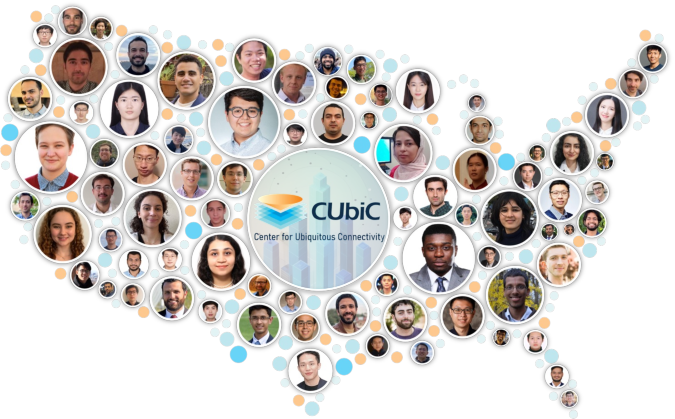
\includegraphics[width=\linewidth]{../../6_figures/ds_fig_cubic.pdf}
    \end{center}
    \caption{Firsthand experience of broadening participation in action at the CUbiC Center under SRC JUMP 2.0 have profoundly shaped my understanding of inclusive practices in STEM education and large-scale research programs.}
    \label{fig:cubic}
    \vspace{-0.5em}
\end{wrapfigure}

As one of the mentors in the Summer Undergraduate Research Experience (SURE) Program at \mySchoolShort{}, I had the opportunity to work with students from historically marginalized groups in STEM education. In one particular instance, I mentored a student who had transferred from a community college and between multiple universities, and have recently returned to higher education after two years exploring other career options. The student had a diverse background in terms of curriculum and research experience, but was eager to narrow down their research interests and get hands on experiments in the lab. In this case, I worked with the student in a more appropriate pace, providing them with the necessary background knowledge and pointers to more resources, and gradually increasing the complexity of the tasks as they felt comfortable. The student was able to present their work at the end of the summer independently. This experience had inspired me to reflect on the boundaries between mentoring and teaching especially in a student's formative years, as the two roles are often intertwined. I am committed to bring together these experiences and thinking into the creation of an inclusive environment where students from all backgrounds can thrive and succeed.

My time at the Center for Ubiquitous Connectivity (CUbiC) under the SRC JUMP 2.0 program has been instrumental in shaping my understanding of outreaching and broadening participation in action. Diversity is a critical priority in CUbiC, as evidenced by the Center featuring a female director, a female theme lead, 6 female principal investigators, alongside over 20\% and growing researchers from underrepresented groups. I have also contributed to increasing the participation of undergraduate and Master's students in the Center's research by creating research projects and hand-on experiences that are appropriate for students at different levels. Furthermore, our pledge and effort to increase diversity in CUbiC have been recognized by the SRC JUMP 2.0 program and used as a model for other JUMP Centers to follow, as shown in Fig.~\ref{fig:cubic}. Participating in the Center's inclusive mentoring and outreach programs has demonstrated to me the utmost importance of such initiatives in a research environment. These experiences have provided me with a solid framework for what I aspire to emulate in establishing my own research group and collaborative projects at \appSchoolDeptShort{}.

In conclusion, it is through the combined efforts\textemdash recognizing the full spectrum of diversity, actively contributing to an inclusive academic culture, and taking every opportunity to educate and inform\textemdash that I aim to fulfill the responsibility that accompanies my educational achievement. I see it as my duty to ensure that the pathways to academic and professional success are accessible to all, and to serve as a mentor for the next generation of scholars and innovators.